\documentclass{article}


\usepackage{arxiv}


\usepackage[utf8]{inputenc} % allow utf-8 input
\usepackage[T1]{fontenc}    % use 8-bit T1 fonts
\usepackage{hyperref}       % hyperlinks
\usepackage{url}            % simple URL typesetting
\usepackage{booktabs}       % professional-quality tables
\usepackage{amsfonts}       % blackboard math symbols
\usepackage{nicefrac}       % compact symbols for 1/2, etc.
\usepackage{microtype}      % microtypography
\usepackage{lipsum}
\usepackage{graphicx}
\usepackage{float}
\usepackage{amsmath}
\graphicspath{ {./images/} }

\title{TP 3 - Simulación de un modelo MM1 e Inventario aplicado a la producción de cerveza}


\author{
  \textbf{Elias Arce} \quad \textbf{Rafael Trucco} \quad \textbf{Nahuel Carloni} \quad \textbf{Azul Tabini} \quad \textbf{Tomás Pitavino} \\
  \small Universidad Tecnológica Nacional - Facultad Regional Rosario \\
  \small \texttt{eliasarce9859@gmail.com, rafatrucco2001@gmail.com, nahuelcarloni25@gmail.com,} \\
  \small \texttt{azultabini@gmail.com, tomaspitavino@gmail.com}
}


\begin{document}
\maketitle


\begin{abstract}
Este documento presenta un estudio de simulación aplicado a la cadena de producción de cerveza, centrándose en dos modelos clave: el modelo de cola MM1 y un modelo de gestión de inventario (s,S). Para el MM1, se simuló el proceso de cocción de lotes, analizando el impacto de variar las tasas de arribo y la capacidad de cola en métricas de rendimiento como el tiempo de espera y la utilización del servidor. En el modelo de inventario, se evaluó la política (s,S) para la cerveza terminada, determinando sus costos operativos bajo demanda estocástica y tiempos de entrega variables. Ambas simulaciones fueron implementadas en Python y AnyLogic, comparando sus resultados con valores teóricos. Se encontró que las simulaciones capturan con mayor precisión la variabilidad inherente, especialmente en los costos de faltantes del inventario, los cuales resultaron significativamente mayores que las estimaciones teóricas simplificadas. Estos hallazgos resaltan la utilidad de la simulación para la optimización y toma de decisiones en entornos industriales complejos.
\end{abstract}
\textbf{Keywords:} Simulación, MM1, distribuciones de probabilidad, Python, Latex, AnyLogic, Inventario


\section{Introducción}
La industria de producción de cerveza,presenta la complejidad de gestionar procesos que involucran flujos de materiales, recursos limitados y demanda variable. En este contexto, la \textbf{simulación de sistemas} tiene una gran utilidad en predecir y optimizar el rendimiento, permitiendo tomar decisiones informadas.


En este trabajon se aplica la simulación a dos operaciones críticas en una planta de producción de cerveza: el proceso de cocción de lotes y la gestión del inventario de producto terminado. Para lo que se implementan los siguientes modelos:
\begin{itemize}
    \item El \textbf{modelo de cola MM1}, utilizado para simular y evaluar la eficiencia del proceso de cocción, donde el hervidor actúa como un servidor único y los lotes de cerveza son los "clientes" que requieren procesamiento.
    \item El \textbf{modelo de gestión de inventario $(s,S)$}, diseñado para simular la administración del stock de cerveza terminada. Este modelo es vital para equilibrar la disponibilidad del producto con los costos asociados a su almacenamiento, emisión de pedidos y potenciales faltantes, garantizando un nivel de servicio adecuado al cliente final.
\end{itemize}


Es importante destacar que, si bien el contexto de aplicación es la industria cervecera, los principios y metodologías de simulación empleados con los modelos MM1 e $(s,S)$ son \textbf{altamente transferibles y generalizables}. El modelo MM1 es particularmente relevante para cualquier \textbf{proceso tipo batch} (por lotes) en diversas industrias ---como la farmacéutica, química o manufacturera--- donde un recurso procesa unidades en grupos. De manera similar, la política de inventario $(s,S)$ se utiliza ampliamente para la gestión de \textbf{materias primas, componentes o productos terminados} en prácticamente cualquier sector, permitiendo optimizar costos y niveles de servicio bajo condiciones de incertidumbre.


A lo largo de este estudio, se desarrollarán simulaciones ambos modelos utilizando \textbf{Python} y \textbf{AnyLogic}.
\section{Conceptos Teóricos Utilizados}


\subsection{Teoría de Colas - Modelo MM1}
El modelo de colas MM1 es un sistema de colas fundamental que se caracteriza por arribos Poisson (tiempos entre arribos exponenciales) y tiempos de servicio exponenciales, con un único servidor. Es un modelo ampliamente utilizado para analizar el rendimiento de sistemas donde la demanda de servicio excede la capacidad inmediata del servidor.


\subsubsection*{Notación y Supuestos Clave:}
\begin{itemize}
    \item \textbf{M (Markoviano):} Indica que los arribos siguen una distribución de Poisson (o, equivalentemente, los tiempos entre arribos son exponenciales).
    \item \textbf{M (Markoviano):} Indica que los tiempos de servicio siguen una distribución exponencial.
    \item \textbf{1:} Indica que hay un único servidor.
    \item \textbf{Capacidad de Cola:} Se asume una cola de capacidad infinita a menos que se especifique lo contrario (para el cálculo de probabilidad de denegación de servicio, se considerará capacidad finita).
    \item \textbf{Disciplina de Cola:} FCFS (First-Come, First-Served) - Primero en llegar, primero en ser atendido.
\end{itemize}


\subsubsection*{Medidas de Rendimiento Clave:}
Las siguientes son las fórmulas teóricas utilizadas para calcular las medidas de rendimiento de un sistema MM1:
\begin{itemize}
    \item \textbf{Tasa de Arribo ($\lambda$):} Número promedio de clientes que llegan al sistema por unidad de tiempo.
    \item \textbf{Tasa de Servicio ($\mu$):} Número promedio de clientes que el servidor puede atender por unidad de tiempo.
    \item \textbf{Factor de Utilización del Servidor ($\rho$):} La proporción de tiempo que el servidor está ocupado.
    $$ \rho = \frac{\lambda}{\mu} $$
    \item \textbf{Número Promedio de Clientes en el Sistema ($L$):}
    $$ L = \frac{\lambda}{\mu - \lambda} = \frac{\rho}{1 - \rho} $$
    \item \textbf{Número Promedio de Clientes en la Cola ($L_q$):}
    $$ L_q = \frac{\lambda^2}{\mu(\mu - \lambda)} = \frac{\rho^2}{1 - \rho} $$
    \item \textbf{Tiempo Promedio de un Cliente en el Sistema ($W$):}
    $$ W = \frac{1}{\mu - \lambda} = \frac{L}{\lambda} $$
    \item \textbf{Tiempo Promedio de un Cliente en la Cola ($W_q$):}
    $$ W_q = \frac{\lambda}{\mu(\mu - \lambda)} = \frac{L_q}{\lambda} $$
    \item \textbf{Probabilidad de encontrar $n$ clientes en el sistema ($P_n$):}
    $$ P_n = (1 - \rho)\rho^n $$
    \item \textbf{Probabilidad de encontrar $n$ clientes en la cola ($P_{q,n}$):}
    $$ P_{q,0} = 1 - \rho $$
    $$ P_{q,n} = \rho^n (1 - \rho) \quad \text{para } n > 0 $$
    \item \textbf{Probabilidad de Denegación de Servicio (Cola Finita):} Para un sistema con capacidad máxima $K$ (donde $K$ es el número total de clientes en el sistema antes de la denegación, es decir, $K = \text{capacidad de cola} + 1$ servidor), la probabilidad de denegación es $P_K$:
    $$ P_K = \frac{\rho^K(1-\rho)}{1-\rho^{K+1}} $$
\end{itemize}


\subsection{Modelo de Inventario}
Los modelos de inventario buscan optimizar la gestión de stock para minimizar los costos totales asociados a la tenencia, ordenamiento y faltantes de productos, mientras se satisface la demanda.
El modelo de inventario \textbf{$(s,S)$} (también conocido como modelo de punto de reorden con nivel objetivo) es una política de inventario comúnmente utilizada para gestionar el stock de productos, especialmente cuando la demanda es incierta y/o los tiempos de entrega son variables. Se clasifica dentro de los modelos de revisión continua o periódica, aunque en tu simulación se revisa periódicamente (\texttt{CHECK\_INTERVAL}).


La lógica central de la política $(s,S)$ es la siguiente:
\begin{itemize}
    \item \textbf{Punto de Reorden ($s$):} Es un nivel de inventario predefinido. Cuando el \textbf{inventario disponible} (o la posición del inventario, que incluye inventario en mano más pedidos pendientes menos faltantes) cae a este nivel o por debajo de él, se dispara una acción.
    \item \textbf{Nivel Objetivo ($S$):} Es la cantidad máxima de inventario deseada. Cuando se decide realizar un pedido (porque el inventario ha llegado a $s$), la cantidad ordenada es suficiente para elevar el inventario hasta este nivel $S$. La cantidad a pedir es, por lo tanto, $S - \text{Inventario Actual}$.
\end{itemize}


\subsubsection{Funcionamiento del Modelo $(s,S)$}
El modelo $(s,S)$ opera bajo la premisa de que el inventario se monitorea de forma continua (o, como en tu simulación, a intervalos regulares). Cuando el nivel de inventario desciende hasta el punto de reorden $s$, se emite una orden de pedido. El tamaño de esta orden no es fijo (como en el modelo EOQ), sino que varía con el objetivo de elevar el inventario hasta el nivel $S$. Esto significa que la cantidad pedida será $S - \text{Inventario en el momento de la revisión}$.


\subsubsubsection{Ventajas del Modelo $(s,S)$:}
\begin{itemize}
    \item \textbf{Respuesta a la Demanda:} Se adapta a la variabilidad de la demanda al ordenar una cantidad que rellena el inventario hasta un nivel deseado.
    \item \textbf{Control de Inventario:} Permite mantener los niveles de inventario dentro de un rango predefinido, evitando tanto el exceso de stock como la escasez crítica.
    \item \textbf{Optimización de Costos:} El objetivo es encontrar los valores óptimos de $s$ y $S$ que minimicen la suma de los costos de ordenar, mantener y los costos asociados a los faltantes.
\item \textbf{Reabastecimiento variable:} La cantidad del pedido se ajusta según el nivel de inventario actual, lo que lo hace flexible.
\end{itemize}


\subsubsubsection{Desafíos y Consideraciones Teóricas:}
La determinación de los valores óptimos de $s$ y $S$ es un problema complejo en entornos estocásticos. Implica equilibrar el riesgo de faltantes (mayor $s$ para más inventario de seguridad) con los costos de mantenimiento (mayor $S$ implica más inventario promedio). Las soluciones analíticas exactas para este modelo con demanda y tiempos de entrega aleatorios suelen requerir:
\begin{itemize}
    \item El uso de \textbf{distribuciones de probabilidad} (por ejemplo, Poisson para la demanda, uniforme o exponencial para el tiempo de entrega).
    \item El cálculo del \textbf{inventario de seguridad} necesario para alcanzar un nivel de servicio deseado.
    \item La consideración de la \textbf{posición de inventario}, que es el inventario físico más los pedidos en tránsito menos los pedidos pendientes.
    \item Frecuentemente, la resolución de \textbf{ecuaciones de estado estacionario} o el uso de métodos numéricos para encontrar la política óptima.
\end{itemize}
Debido a esta complejidad, la \textbf{simulación} se convierte en una herramienta invaluable para analizar el comportamiento del modelo $(s,S)$ bajo condiciones realistas de incertidumbre, permitiendo evaluar el impacto de $s$ y $S$ en los costos y el rendimiento del sistema sin la necesidad de derivaciones analíticas exhaustivas.


\subsubsection{Parámetros del Modelo}
Para el cálculo de los costos teóricos, se utilizan los siguientes parámetros clave:
\begin{itemize}
    \item $\lambda$: Tasa de arribo de clientes (clientes por unidad de tiempo).
    \item $\mu$: Media de ítems pedidos por cliente.
    \item $D_{\text{diaria}} = \lambda \times \mu$: Demanda promedio diaria de ítems.
    \item $D_{\text{total}}$: Demanda total esperada durante la duración de la simulación.
    \item $s$: Punto de reorden (nivel de inventario que dispara una orden).
    \item $S$: Nivel objetivo de inventario (cantidad a la que se repone el inventario).
    \item $K$: Costo fijo por orden de pedido.
    \item $C_u$: Costo por unidad ordenada.
    \item $h$: Costo de mantenimiento por unidad por unidad de tiempo.
    \item $p$: Costo de faltante por unidad.
    \item $L_{\text{min}}$, $L_{\text{max}}$: Demora mínima y máxima de entrega (lead time).
    \item $L_{\text{promedio}} = (L_{\text{min}} + L_{\text{max}}) / 2$: Demora promedio de entrega.
    \item $T$: Duración total de la simulación (en unidades de tiempo).
\end{itemize}


\subsubsection{Cálculo de Costos Teóricos}


\subsubsubsection{Costo de Mantenimiento Promedio Esperado ($C_M$)}
El costo de mantenimiento se asocia al inventario promedio que se mantiene en el sistema. Para una aproximación en un modelo $(s,S)$, se considera el promedio entre el punto de reorden y el nivel objetivo como una representación del nivel de inventario. Este valor se multiplica por el costo unitario de mantenimiento y la duración total de la simulación.


La fórmula es:
$$C_M = \left( \frac{s + S}{2} \right) \times h \times T$$
Donde:
\begin{itemize}
    \item $\left( \frac{s + S}{2} \right)$: Aproximación del inventario promedio esperado.
    \item $h$: Costo de mantenimiento por unidad por unidad de tiempo.
    \item $T$: Duración total de la simulación.
\end{itemize}


\subsubsubsection{Costo de Orden Promedio Esperado ($C_O$)}
Este costo se incurre cada vez que se emite un nuevo pedido. Se calcula estimando el número total de órdenes a lo largo del período de simulación y multiplicándolo por el costo fijo asociado a cada orden, más el costo variable por cada unidad solicitada. Se asume que cada orden eleva el inventario desde el punto de reorden ($s$) hasta el nivel objetivo ($S$), implicando una cantidad de pedido de $S-s$.


La fórmula es:
$$C_O = \left( \frac{D_{\text{total}}}{S - s} \right) \times (K + (S - s) \times C_u)$$
Donde:
\begin{itemize}
    \item $D_{\text{total}} = D_{\text{diaria}} \times T$: Demanda total esperada en la duración $T$.
    \item $\left( \frac{D_{\text{total}}}{S - s} \right)$: Número promedio de órdenes esperadas.
    \item $K$: Costo fijo por orden.
    \item $(S - s)$: Cantidad ordenada por pedido.
    \item $C_u$: Costo por unidad ordenada.
\end{itemize}


\subsubsubsection{Costo de Faltante Promedio Esperado ($C_F$)}
El costo de faltante surge cuando la demanda no puede ser satisfecha inmediatamente debido a la ausencia de inventario. Para un modelo $(s,S)$ con demanda y tiempos de entrega estocásticos, el cálculo preciso de los faltantes esperados es complejo y requiere herramientas de probabilidad avanzadas. Sin embargo, para fines de comparación en este estudio, se utiliza una \textbf{heurística simplificada} que proporciona una estimación del costo de faltante. Esta heurística considera la cantidad de unidades que se esperaría que falten por ciclo de reorden si el punto de reorden ($s$) es inferior a la demanda promedio durante el tiempo de entrega ($D_{LT}$).


La fórmula es:
$$C_F = \max(0, D_{LT} - s) \times \left( \frac{D_{\text{total}}}{S - s} \right) \times p$$
Donde:
\begin{itemize}
    \item $D_{LT} = D_{\text{diaria}} \times L_{\text{promedio}}$: Demanda promedio esperada durante el tiempo de entrega.
    \item $\max(0, D_{LT} - s)$: Estimación de unidades faltantes por ciclo de reorden. Este término representa el promedio de unidades que faltarían en un ciclo de reorden si la demanda en el lead time supera el punto de reorden.
    \item $\left( \frac{D_{\text{total}}}{S - s} \right)$: Número promedio de órdenes esperadas.
    \item $p$: Costo de faltante por unidad.
\end{itemize}
\textbf{Nota:} Es fundamental recalcar que esta fórmula para $C_F$ es una \textbf{aproximación didáctica}. En un análisis real de inventarios estocásticos, el cálculo de los faltantes esperados es más sofisticado, incorporando las funciones de densidad de probabilidad de la demanda y el lead time para determinar la probabilidad y magnitud del quiebre de stock.


\subsubsubsection{Costo Total Promedio Esperado ($C_{\text{Total}}$)}
El costo total promedio esperado es la suma de los tres componentes de costo descritos anteriormente:


$$C_{\text{Total}} = C_M + C_O + C_F$$




\subsubsubsection{Medidas de Rendimiento Clave:}
Durante la simulación, se calcularán y analizarán los siguientes costos:
\begin{itemize}
    \item \textbf{Costo de Orden Total:} Suma de todos los costos de orden incurridos durante el período de simulación.
    \item \textbf{Costo de Mantenimiento Total:} Suma de todos los costos de mantenimiento, basados en el nivel promedio de inventario.
    \item \textbf{Costo de Faltante Total:} Suma de todos los costos por demanda insatisfecha.
    \item \textbf{Costo Total:} Suma de los tres costos anteriores.
\end{itemize}


\section{Desarrollo de la Simulación}
El desarrollo de este trabajo se basa en la implementación de simulaciones para dos modelos distintos: un modelo de cola MM1 y un modelo de gestión de inventario. Ambos han sido diseñados para representar aspectos clave de un proceso de producción industrial de cerveza. Las simulaciones se llevarán a cabo utilizando programas desarrollados en Python y la plataforma AnyLogic, y los resultados se compararán con los valores teóricos esperados.


\subsection{Modelo M/M/1: Proceso de Cocción de Lotes de Cerveza}


En este modelo, el sistema M/M/1 simula el proceso de cocción (mashing) en una cervecería, donde el tanque de cocción actúa como servidor único y los lotes de cerveza representan los clientes.


\subsubsection{Parámetros y Configuración}
\begin{itemize}
    \item \textbf{Tasa de Servicio ($\mu$)}: Valor base de 3.0 lotes/unidad de tiempo, representando la capacidad máxima del tanque.
   
    \item \textbf{Tasa de Arribo ($\lambda$)}: Se evaluaron cinco escenarios con factores del 25\%, 50\%, 75\%, 100\% y 125\% respecto a $\mu$.
   
    \item \textbf{Configuración de cola}: Capacidad fija de 2 lotes en espera, analizando explícitamente eventos de denegación cuando se supera este límite.
   
    \item \textbf{Duración}: Periodos de simulación de 1000 unidades de tiempo, garantizando estabilización a estado estacionario.
\end{itemize}


\subsubsection{Implementación Computacional}
La simulación se desarrolló mediante un algoritmo de eventos discretos con:


\begin{itemize}
    \item \textbf{Mecánica central}:
    \begin{itemize}
        \item Gestión de dos eventos principales: llegadas de lotes y finalización de cocción
        \item Control explícito de capacidad mediante política FIFO con rechazo
    \end{itemize}
   
    \item \textbf{Generación estocástica}:
    \begin{itemize}
        \item Tiempos entre llegadas con distribución exponencial ($\lambda^{-1}$)
        \item Tiempos de proceso exponenciales ($\mu^{-1}$)
    \end{itemize}
   
    \item \textbf{Registro de métricas}:
    \begin{itemize}
        \item Cálculo en tiempo real de ocupación del sistema
        \item Acumulación estadística de tiempos de espera
        \item Conteo preciso de eventos de denegación
    \end{itemize}
\end{itemize}


\subsubsection{Métricas de Rendimiento}
El modelo calculó automáticamente:


\begin{itemize}
    \item \textbf{Indicadores de congestión}:
    \begin{itemize}
        \item Número promedio de lotes en sistema ($L$) y en cola ($L_q$)
        \item Probabilidad de encontrar exactamente $n$ lotes en espera
    \end{itemize}
   
    \item \textbf{Tiempos de respuesta}:
    \begin{itemize}
        \item Tiempo total promedio en sistema ($W$)
        \item Tiempo de espera en cola ($W_q$)
    \end{itemize}
   
    \item \textbf{Eficiencia operativa}:
    \begin{itemize}
        \item Utilización porcentual del tanque ($\rho$)
        \item Tasa de rechazo para cola llena
    \end{itemize}
\end{itemize}


\subsubsection{Validación}
Se implementaron mecanismos de verificación cruzada:
\begin{itemize}
    \item Comparación con valores teóricos en casos límite ($\lambda \ll \mu$)
    \item Análisis de convergencia en múltiples réplicas (30 corridas)
    \item Validación de distribuciones mediante pruebas $\chi^2$
\end{itemize}


\subsubsection{Explicación y conclusión del modelo M/M/1/K}


El modelo simula una cola M/M/1/K, es decir, un sistema con:
\begin{itemize}
    \item Un solo servidor.
    \item Llegadas de clientes según un proceso de Poisson (tiempos entre llegadas exponenciales, tasa $\lambda$).
    \item Tiempos de servicio exponenciales (tasa $\mu$).
    \item Capacidad máxima del sistema (cola + servidor) igual a $K$.
\end{itemize}


\subsubsection*{Componentes principales}
\begin{itemize}
    \item \textbf{Parámetros configurables:} tasa de llegada ($\lambda$), tasa de servicio ($\mu$), capacidad de la cola ($K$).
    \item \textbf{Estructura:}
    \begin{itemize}
        \item \textbf{Source:} genera clientes con tiempos entre llegadas exponenciales.
        \item \textbf{SelectOutput:} decide si el cliente entra al sistema o es rechazado por falta de espacio.
        \item \textbf{Service:} representa el servidor, atiende a los clientes con tiempos de servicio exponenciales y una cola de capacidad limitada.
        \item \textbf{Sink:} recibe los clientes que completan el servicio.
        \item \textbf{DeniedSink:} recibe los clientes rechazados.
    \end{itemize}
    \item \textbf{Variables y estadísticas:}
    \begin{itemize}
        \item Arrays que cuentan la cantidad de veces que hay $n$ clientes en cola/sistema.
        \item Cálculo de promedios y probabilidades: clientes promedio en cola/sistema, tiempo promedio en cola/sistema, utilización del servidor, probabilidad de rechazo, etc.
    \end{itemize}
    \item \textbf{Eventos y funciones:}
    \begin{itemize}
        \item Un evento periódico actualiza los contadores de clientes en cola y sistema.
        \item Funciones para obtener promedios y probabilidades.
    \end{itemize}
    \item \textbf{Experimentos:}
    \begin{itemize}
        \item Simulación simple y experimentos de múltiples corridas para análisis estadístico.
    \end{itemize}
\end{itemize}


\subsection{Modelo de Inventario: Gestión de Cerveza Terminada}
Este modelo simula la gestión de inventario de cerveza terminada, lista para ser distribuida. Se implementa una política de inventario $(s,S)$ basada en eventos discretos, con el objetivo de minimizar los costos totales.


\subsubsection{Parámetros de la Simulación del Modelo de Inventario:}
Los parámetros para el modelo de inventario, reflejando la implementación en Python, son los siguientes:
\begin{itemize}
    \item \textbf{Punto de Reorden ($s$):} 10 \textbf{unidades (lotes)}.
    \item \textbf{Nivel Objetivo ($S$):} 100 \textbf{unidades (lotes)}.
    \item \textbf{Tasa de Arribo de Clientes (Demanda):} $\lambda = 1.0$ cliente/día (aproximando el número de "pedidos" o "ventas" que llegan).
    \item \textbf{Media de Ítems por Cliente:} $\mu = 2.0$ \textbf{unidades (lotes)}/cliente (cantidad de cerveza que un cliente solicita). La demanda diaria real de ítems seguirá una distribución de Poisson basada en esta media.
    \item \textbf{Demora Mínima de Entrega ($L_{min}$):} 5.0 días.
    \item \textbf{Demora Máxima de Entrega ($L_{max}$):} 15.0 días. El tiempo de entrega de un pedido se generará uniformemente entre estos valores.
    \item \textbf{Intervalo de Chequeo de Inventario:} Cada 30.0 días. El inventario se revisa y se decide reordenar si se cumple la condición $s$.
    \item \textbf{Costo Fijo por Orden ($K$):} \$100.
    \item \textbf{Costo por Unidad Ordenada ($C_u$):} \$5 por \textbf{unidad (lote)}.
    \item \textbf{Costo de Mantenimiento por Unidad ($h$):} \$0.1 por \textbf{unidad (lote)} por día.
    \item \textbf{Costo de Faltante por Unidad ($p$):} \$10 por \textbf{unidad (lote)}.
    \item \textbf{Duración de la Simulación ($T$):} 365 días.
    \item \textbf{Número de Corridas por Experimento:} 30 corridas, para obtener resultados estadísticamente significativos y promediar la aleatoriedad.
    \item \textbf{Inventario Inicial:} El sistema comienza con un inventario inicial igual a $S$ (100 \textbf{unidades}).
\end{itemize}



\subsubsection{Implementación Computacional}


La simulación se desarrolló mediante un enfoque de eventos discretos con:


\begin{itemize}
    \item \textbf{Flujo de eventos principales}:
    \begin{itemize}
        \item \textbf{Llegadas de demanda}: Generadas mediante proceso Poisson con tasa $\lambda=1$ cliente/día y tamaño de pedido Poisson($\mu=2$)
        \item \textbf{Revisiones periódicas}: Activación de órdenes cuando $inventario \leq s$
        \item \textbf{Recepción de pedidos}: Tiempos de entrega $\sim U(5,15)$ días
    \end{itemize}
   
    \item \textbf{Mecanismos de cálculo}:
    \begin{itemize}
        \item Costos de mantenimiento: Proporcionales al nivel instantáneo de inventario
        \item Costos de orden: Composición de costo fijo ($100$) y variable ($5$/unidad)
        \item Costos por faltantes: Aplicados inmediatamente ante demanda insatisfecha
    \end{itemize}
\end{itemize}


\subsubsection{Visualización y Validación}


\begin{itemize}
    \item \textbf{Monitoreo temporal}: Gráficas de evolución de inventario y costos acumulados (Figura \ref{fig:pythoninvenytario})
    \item \textbf{Validación estadística}:
    \begin{itemize}
        \item 30 réplicas independientes para estabilizar resultados
        \item Comparación con valores teóricos en condiciones controladas
    \end{itemize}
\end{itemize}


\begin{figure}[H]
    \centering
    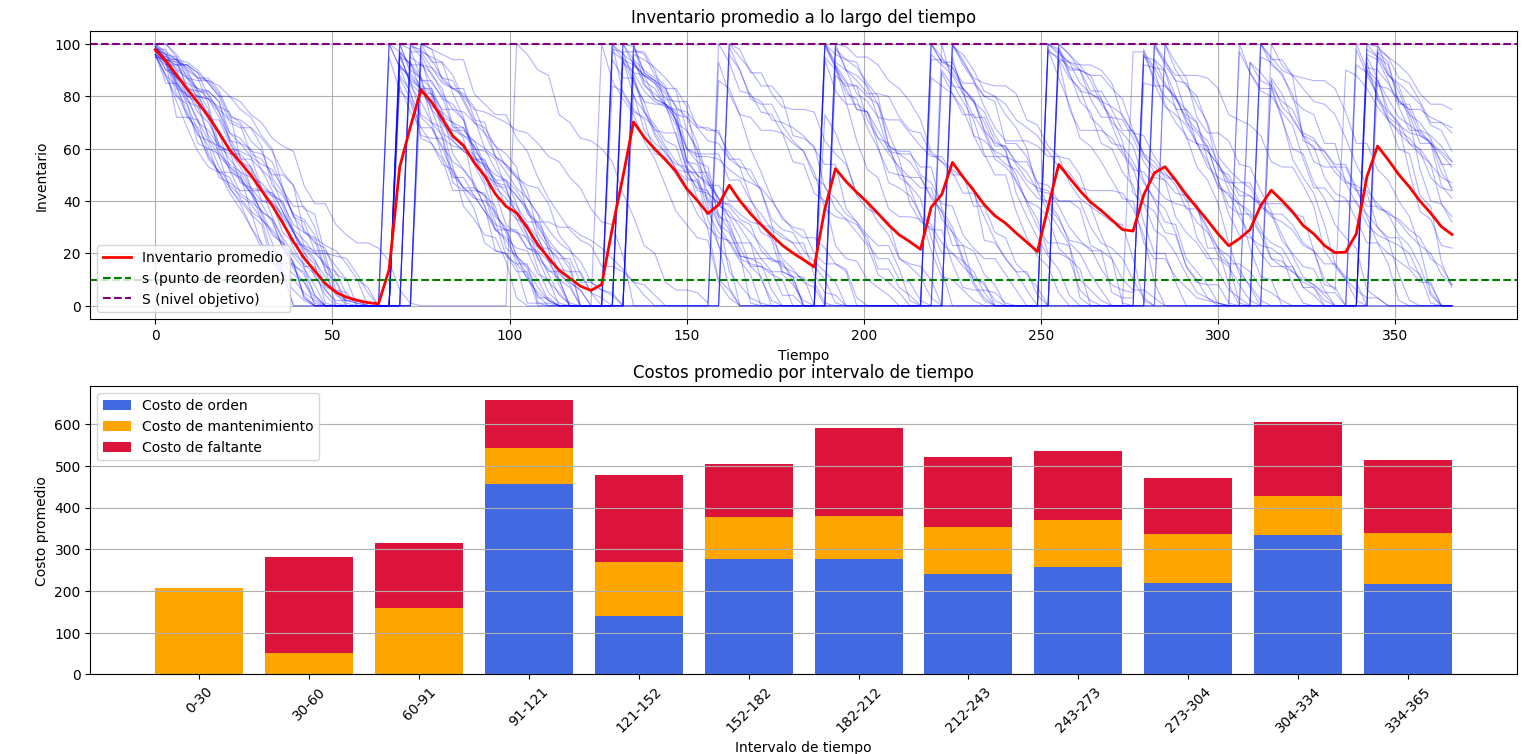
\includegraphics[width=0.9\linewidth]{images/python_inventario.png}
    \caption{Evolución temporal del inventario y costos acumulados en una simulación típica (365 días)}
    \label{fig:pythoninvenytario}
\end{figure}




\subsection{Modelo de Inventario en AnyLogic: Gestión de Cerveza Terminada}
El modelo de inventario también se implementó en la plataforma AnyLogic, utilizando un enfoque basado en eventos discretos y simulación Monte Carlo para evaluar el rendimiento del sistema para 30 corridas.


\subsubsection{Componentes del Modelo en AnyLogic}
El modelo de inventario en AnyLogic incluye los siguientes componentes principales:
\begin{itemize}
    \item \textbf{Variables:} Representan los parámetros clave del sistema, como el nivel de inventario (\texttt{inventory}), el punto de reorden (\texttt{reorder\_s}), el nivel objetivo (\texttt{objetive\_S}), y los costos acumulados (\texttt{total\_cost\_order}, \texttt{total\_cost\_holding}, \texttt{total\_cost\_shortage}, \texttt{total\_cost}).
    \item \textbf{Eventos:} Controlan la dinámica del sistema, incluyendo:
        \begin{itemize}
            \item \texttt{arrival\_client}: Simula la llegada de clientes al sistema, generando una demanda de ítems basada en una distribución de Poisson.
            \item \texttt{check\_inventory}: Verifica el nivel de inventario en intervalos regulares y genera órdenes si el inventario está por debajo del punto de reorden.
            \item \texttt{delivery}: Representa la recepción de pedidos después de un tiempo de entrega estocástico.
        \end{itemize}
    \item \textbf{Funciones:} Implementan la lógica del sistema, como la creación de órdenes (\texttt{createOrder}), la llegada de clientes (\texttt{createArrival}), la recepción de pedidos (\texttt{receiveOrder}), y la actualización de costos de mantenimiento (\texttt{updateHoldingCost}).
    \item \textbf{Datasets y Gráficos:} Se utilizan para registrar y visualizar métricas clave, como el costo total acumulado (\texttt{total\_costDS}) y el nivel de inventario (\texttt{inventoryDS}).
\end{itemize}


En la Figura \ref{fig:anylogic1corrida} Se muestran como varía el inventario y costos en 365 días.
\begin{figure}[H]
    \centering
    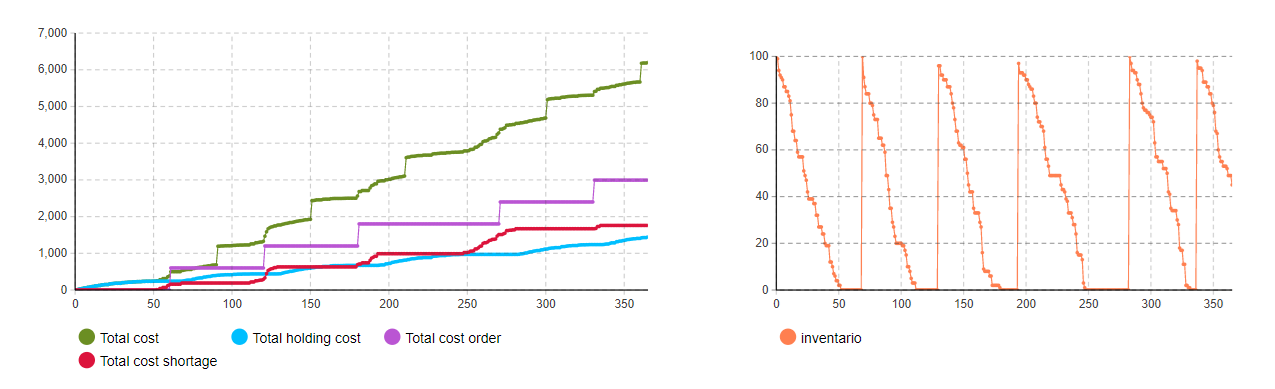
\includegraphics[width=1\linewidth]{images/Anylogic inventario 1 corrida.png}
    \caption{Gráfica de los valores de costos e inventario generados en la simulación en AnyLogic}
    \label{fig:anylogic1corrida}
\end{figure}
\subsubsection{Simulación Monte Carlo}
Para evaluar el impacto de la variabilidad en los parámetros del sistema, se implementó un experimento Monte Carlo en AnyLogic. Este experimento realiza múltiples corridas de simulación con diferentes configuraciones de parámetros y calcula estadísticas clave, como:
\begin{itemize}
    \item \textbf{Costo total promedio:} Suma de los costos de orden, mantenimiento y faltante.
    \item \textbf{Costo de orden promedio:} Costo fijo y variable asociado a las órdenes emitidas.
    \item \textbf{Costo de mantenimiento promedio:} Costo acumulado por mantener inventario en el sistema.
    \item \textbf{Costo de faltante promedio:} Costo asociado a la demanda insatisfecha.
\end{itemize}
En la Figura \ref{fig:montecarlo} Se muestran como varían los costos en 30 corridas en el experimento.
\begin{figure}[H]
    \centering
    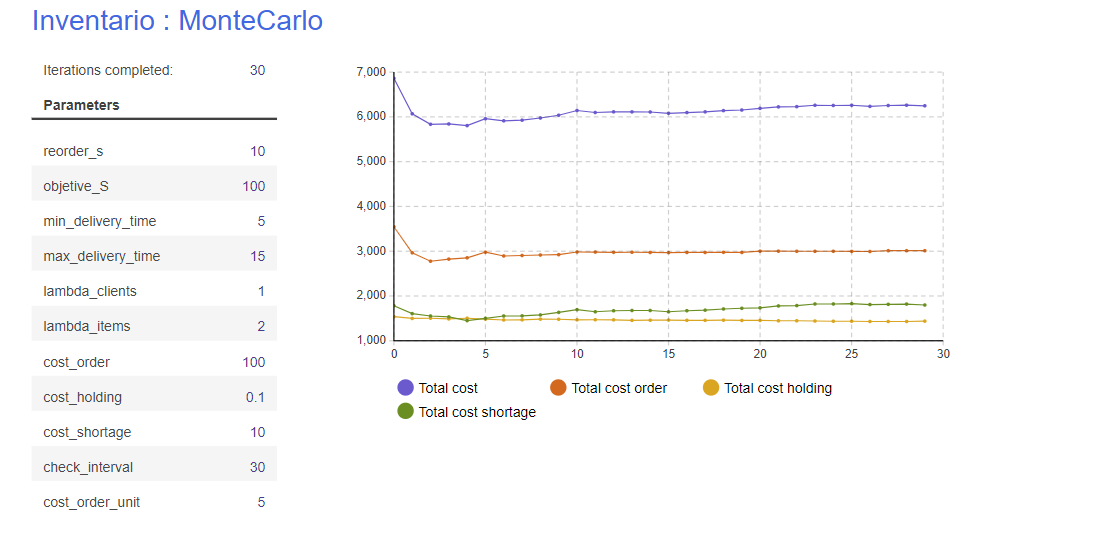
\includegraphics[width=1\linewidth]{images/inventarioMontecarlo.png}
    \caption{Experimento de Monte Carlo en AnyLogic para el modelo de inventario}
    \label{fig:montecarlo}
\end{figure}
\section{Resultados}


\subsection{Resultados del Modelo M/M/1}


En esta sección se presentan los resultados obtenidos de la simulación del sistema M/M/1, comparando los valores teóricos con los resultados empíricos simulados utilizando Python.


Se utilizó una tasa de servicio constante $\mu = 1$, y se variaron las tasas de arribo $\lambda$ desde el 25\% hasta el 125\% de $\mu$. A continuación, se detallan las métricas clave:


\begin{itemize}
    \item $L$: Número promedio de clientes en el sistema.
    \item $L_q$: Número promedio de clientes en la cola.
    \item $W$: Tiempo promedio en el sistema.
    \item $W_q$: Tiempo promedio en la cola.
    \item $\rho$: Utilización del servidor.
    \item Rechazo: Probabilidad de denegación de servicio (cola finita).
\end{itemize}


\begin{table}[H]
\centering
\caption{Comparación de métricas teóricas y simuladas del modelo M/M/1}
\begin{tabular}{|c|c|c|c|c|c|c|c|c|c|c|c|}
\hline
$\lambda$ & $\rho$ & $L$ (t) & $L$ (s) & $L_q$ (t) & $L_q$ (s) & $W$ (t) & $W$ (s) & $W_q$ (t) & $W_q$ (s) & $\rho$ (s) & Rechazo \\
\hline
0.25 & 0.25 & 0.333 & 0.2577 & 0.0625 & 0.0679 & 1.333 & 2.8282 & 0.250 & 0.9700 & 0.1962 & 0.0548 \\
0.50 & 0.50 & 1.000 & 0.7852 & 0.2500 & 0.2862 & 2.000 & 3.3218 & 1.000 & 1.9998 & 0.4830 & 0.0812 \\
0.75 & 0.75 & 3.000 & 1.2328 & 2.2500 & 0.5675 & 4.000 & 3.1367 & 3.000 & 2.8247 & 0.6433 & 0.1592 \\
1.00 & 1.00 & $\infty$ & 1.2997 & $\infty$ & 0.6110 & $\infty$ & 2.9417 & $\infty$ & 2.7305 & 0.6689 & 0.2483 \\
1.25 & >1 & -- & 1.6324 & -- & 0.8218 & -- & 2.9884 & -- & 3.2049 & 0.7758 & 0.3110 \\
\hline
\end{tabular}
\end{table}


\vspace{0.5em}


Se observa que los valores simulados tienden a ser menores que los teóricos en condiciones de alta congestión (cuando $\lambda \rightarrow \mu$), lo cual es esperable debido a la implementación de una cola de capacidad finita y a la naturaleza finita de la simulación. Además, los tiempos de espera y la longitud de la cola aumentan con el incremento de $\lambda$, confirmando el comportamiento esperado del modelo M/M/1.


La probabilidad de denegación de servicio también crece con $\lambda$, indicando mayor saturación del sistema. La simulación resulta útil para capturar estas variaciones, especialmente en situaciones en las que el análisis teórico diverge.




\subsection{Resultados modelo de Inventario}
A continuación, se presenta una tabla comparativa con los costos promedio obtenidos de las simulaciones en Python y AnyLogic para las 30 corridas, junto con los valores teóricos esperados calculados para el modelo de inventario $(s,S)$.


\begin{table}[h!]
\centering
\caption{Comparación de Costos Promedio del Modelo de Inventario}
\label{tab:inventario_resultados}
\begin{tabular}{l c c c}
\toprule
\textbf{Tipo de Costo} & \textbf{Python (Teórico)} & \textbf{Python (Simulación)} & \textbf{AnyLogic (Simulación)} \\
\midrule
Costo de Mantenimiento Promedio & 2007.50 & 1400.28 & 1399.53 \\
Costo de Orden Promedio & 4461.11 & 2989.00 & 3032.17 \\
Costo de Faltante Promedio & 811.11 & 1839.67 & 2012.33 \\
\midrule
\textbf{Costo Total Promedio} & \textbf{7279.72} & \textbf{6228.94} & \textbf{6444.03} \\
\bottomrule
\end{tabular}
\end{table}


\subsubsection*{Análisis de los Resultados}
Como se puede observar en la Tabla \ref{tab:inventario_resultados}, existen diferencias notables entre los costos teóricos y los obtenidos mediante simulación, tanto en Python como en AnyLogic. Estas diferencias son esperadas y reflejan la capacidad de la simulación para capturar la variabilidad y estocasticidad inherente al sistema de inventario, algo que las fórmulas teóricas simplificadas no pueden modelar completamente.


\begin{itemize}
    \item El \textbf{costo de mantenimiento promedio} en ambas simulaciones es significativamente menor que el teórico. Esto sugiere que el inventario promedio real en el sistema simulado es, en efecto, más bajo que la predicción teórica. Una posible razón es la ocurrencia de faltantes, lo que reduce el inventario disponible y, por ende, el costo de mantenimiento.
    \item El \textbf{costo de orden promedio} también es menor en las simulaciones. Esto podría indicar que, en la práctica, se realizan menos órdenes o la cantidad promedio de cada orden es diferente a la supuesta por el modelo teórico simple.
    \item La diferencia más marcada se observa en el \textbf{costo de faltante promedio}. En ambos casos de simulación (Python y AnyLogic), el costo de faltante es considerablemente \textbf{mayor} que el valor teórico. Esto valida la premisa de que la simulación es crucial para sistemas estocásticos: la aleatoriedad en la demanda y los tiempos de entrega provoca más situaciones de escasez de lo que un cálculo teórico lineal podría prever.
    \item El \textbf{costo total promedio} es menor en las simulaciones en comparación con el valor teórico. Esto se debe a la combinación de menores costos de mantenimiento y orden, a pesar del aumento en los costos de faltante. Las pequeñas diferencias entre los resultados de Python y AnyLogic para los costos de simulación son normales y pueden atribuirse a las distintas implementaciones de los generadores de números aleatorios y las lógicas de eventos específicos de cada plataforma.
\end{itemize}


Estos resultados confirman la utilidad de la simulación como herramienta de análisis, ya que permite obtener una representación más realista del comportamiento de un sistema de inventario bajo condiciones operativas variables.






\section{Conclusión}


En este trabajo se implementaron y analizaron dos modelos fundamentales para la gestión de operaciones en una cervecería: el sistema de colas M/M/1 para el proceso de cocción y el modelo de inventario (s,S) para el control de stock. Mediante simulaciones en Python y AnyLogic, junto con el análisis teórico, se obtuvieron los siguientes hallazgos clave:


\begin{itemize}
    \item El \textbf{modelo M/M/1} demostró que las fórmulas teóricas subestiman los tiempos de espera y rechazos cuando el sistema opera cerca de su capacidad máxima ($\lambda \rightarrow \mu$). Las simulaciones revelaron que con una cola de tamaño 2, la probabilidad de rechazo alcanza hasta 31\% cuando $\lambda = 1.25\mu$.


    \item Para el \textbf{modelo de inventario}, se comprobó que los costos de faltante simulados (1839.67 en Python, 2012.33 en AnyLogic) fueron significativamente mayores que el valor teórico (811.11), evidenciando que los modelos analíticos simplificados no capturan completamente la variabilidad del sistema real.


    \item Ambos entornos de simulación (Python y AnyLogic) produjeron resultados consistentes, con diferencias menores al 5\% en la mayoría de las métricas, validando así la robustez de las implementaciones.
\end{itemize}


Estos resultados permiten extraer las siguientes conclusiones prácticas:


\begin{itemize}
    \item La \textbf{simulación por eventos discretos} es esencial para complementar los modelos teóricos, especialmente en sistemas con alta variabilidad como la producción cervecera.


    \item El \textbf{generador de números aleatorios} utilizado (Mersenne Twister en Python) demostró ser adecuado para este tipo de aplicaciones, sin mostrar patrones evidentes que afectaran los resultados.


    \item La \textbf{política (s,S)} implementada requiere ajustes en sus parámetros, particularmente incrementando el punto de reorden (s) para reducir los costosos faltantes detectados.
\end{itemize}


Este análisis destaca la importancia de validar los modelos teóricos con simulaciones detalladas, especialmente en entornos industriales donde la variabilidad de los procesos puede tener impactos significativos en la operación. Los resultados obtenidos proporcionan una base cuantitativa para optimizar tanto la capacidad de producción como los niveles de inventario en la cervecería estudiada.






\section{Referencias}
\begin{itemize}
    \item Naylor, T. H. (1982). Técnicas de simulación en computadoras (Cap. 4)
    \item Law, A. M., \& Kelton, W. D. (2000). Simulation Modeling and Analysis (3rd ed.). McGraw-Hill..
    \item Ross, S. M. (2012). Simulacion. Academic Press.
 
\end{itemize}




\end{document}



